\section{Метод конфигураций}

\begin{itemize}
    \item {\bfseries Класс задач:} безусловная оптимизация
    
    
    \item {\bfseries Формулировка задачи:} Найти минимум функции 2-ух переменных $f(x1, x2)$ методом кофигурации.
    
    
    \item {\bfseries Что вычисляется в процессе решения:}
    В процессе итерации находятся точки базиса, в которых происходит исследующий поиск и поиск по образцу.
    
    
    \item {\bfseries Алгоритм:}
    {\it Описание алгоритма:}
    \begin{enumerate}
        \item Задается начальная точка $x^0 = (x^{0}_1, x^{0}_2, ..., x^{0}_n)$ и начальные значения приращений $dx^{0}_1, dx^{0}_2, ...,  dx^{0}_n$, а также минимальная длина шага $\xi$ для останова и необязательный параметр останова - максимальное количество иттераций $N_{max}$. Для корректной работы алгоритма $dx^{0}_i > \xi$ для $\forall i \in \{1, ..., n\}$. Точка $x^{0}$ называется точкой старого базиса.
        
        \item Проводится исследующий поиск, в результате которого каждого координата новой точки $x^{k + 1}$ вычисляется по алгоритму:
        \begin{enumerate}
        	\item Для $\forall i \in \{1, ..., n\}$: \\
            \begin{equation*}
                x^{k+1}_{i} =
                \begin{cases}
                    x^{k}_{i} + dx^{k}_i, if \quad f(x^{k}_{1}, ..., x^{k}_{i}+ dx^{k}_i, ..., x^{k}_{n}) < f(x^{k}_1, ..., x^{k}_{i}, ..., x^{j}_{n})
                    \\
                    x^{k}_{i} - dx^{k}_i, if \quad f(x^{k}_{1}, ..., x^{k}_{i} - dx^{k}_i, ..., x^{k}_{n}) < min(f(x^{k}_{1}, ..., x^{k}_{i}, ..., x^{k}_{n}), f(x^{k}_1, ..., x^{k}_{i} + dx^{k}_i, ..., x^{k}_{n}))
                    \\
                    x^{k}_{i}, otherwise
                \end{cases}
            \end{equation*}
        \end{enumerate}
        В результате исследующего поиска получается точка $x^{k + 1}$.\\
        Если при этом $x^{k + 1} \neq x^{k}$, то $x^{k + 1}$ - точка нового базиса.\\
        Если $x^{k + 1} = x^{k}$, то исследующий поиск неудачен. В этом случае необходимо уменьшить значения приращений $dx^{j}_1, dx^{j}_2, ...,  dx^{j}_n$ и повторить исследующий поиск.\\
        
        \item Из точки нового базиса может быть:
            \begin{enumerate}
                \item продолжен исследующий поиск со старыми или новыми значения приращений (шаг 2) алгоритма).
                \item проведен поиск по образцу по алгоритму: $x^{(obr)} = x^k + t_{k}(x^k - x^{k - 1})$, , где $t_k$ - параметр движения(зависит от реализаций, обычно $t_k = 2$).
            \end{enumerate}
        %\begin{enumerate}

        В точке $x^{(obr)}$ значение функции не вычисляется, из этой точки проводится исследующий поиск, в результате которого получается точка $x^{(ip)}$.\\

        Если $x^{(ip)} \neq x^{(obr)}$, то точка $x^{k + 1} = x^{(ip)}$ становится точкой нового базиса, а $x^{k}$ - точкой старого базиса. Если $x^{(ip)} = x^{(obr)}$, то поиск по образцу считается неудачным, точки $x^{(ip)}, x^{(obr)}$ - аннулируются, при этом точка $x^{k}$ остается точкой нового базиса, а $x^{k - 1}$ - точкой старого базиса.\\

        \item Процедура 3) повторяется до выполнения критерия окончания счета.\\

        \underline{Основной критерий окончания метода:} $dx^{k} \leqslant \xi$, $dy^{k} \leqslant \xi$\\

        \underline{Изменяемый параметр метода:} величины приращений $dx^{k}, dy^{k}$. 
       % \end{enumerate}
    \end{enumerate} 
    
    
    \item {\bfseries 1-ая итерация:} \\
    $f(x_1, x_2) = 5x^{2}_{1} + 3x_{1}x_{2} + 6x^{2}_{2} + 2x_1 + x_2 + 9$ \\ 
    $\xi = 0.01$ \\
    $N_{max} = 8$ \\
    $j = 0$ \\
    $x^{0}_1 = 11$, $x^{0}_2 = 7$ \\
    $dx^{0}_{1} = 1$, $dx^{0}_{2} = 1$\\
    
    {\it Делаем исследующий поиск}: \\
    $dx^{0}_{1} = 1 > 0.01 = \xi$\\
    $dx^{0}_{2} = 1 > 0.01 = \xi$ \\
    $j < N_{max}$, значит критерий останова не выполнен. \\
    
    $f(x^{j}_1, x^{j}_2) = 5\cdot121 + 3\cdot77 + 6\cdot49 + 22 + 7 + 9 = 1168$
    \begin{enumerate}
        \item Для $x_1$: \\
        $f(x^{j}_1 + 1, x^{j}_2) = 5\cdot144 + 3\cdot84 + 6\cdot49 + 24 + 7 + 9 = 1306 > f(x^{j}_1, x^{j}_2)$ \\ 
        $f(x^{j}_1 - 1, x^{j}_2) = 5\cdot100 + 3\cdot70 + 6\cdot49 + 20 + 7 + 9 = 1040 < f(x^{j}_1, x^{j}_2)$ \\
        Значит $x^{j + 1}_1 = x^{j}_1 - 1 = 11 - 1 = 10$
        \item Для $x_2$: \\
        $f(x^{j}_1, x^{j}_2 + 1) = 5\cdot121 + 3\cdot88 + 6\cdot64 + 22 + 8 + 9 = 1292 > f(x^{j}_1, x^{j}_2)$ \\
        $f(x^{j}_1, x^{j}_2 - 1) = 5\cdot121 + 3\cdot66 + 6\cdot36 + 22 + 6 + 9 = 1056 < f(x^{j}_1, x^{j}_2)$ \\
        Значит, $x^{j + 1}_2 = x^{j}_2 - 1 = 7 - 1 = 6$
    \end{enumerate}
    $dx^{j + 1}_{1} = dx^{j}_{1} = 1, dx^{j + 1}_{2} = dx^{j}_{2}  = 1$\\
    $j = j + 1 = 1$ \\
    $x^1 = (10, \quad 6)$ \\
    {\it Конец первой итерации.}
    
    \item {\bfseries Результат компьютерных вычислений:} \\
    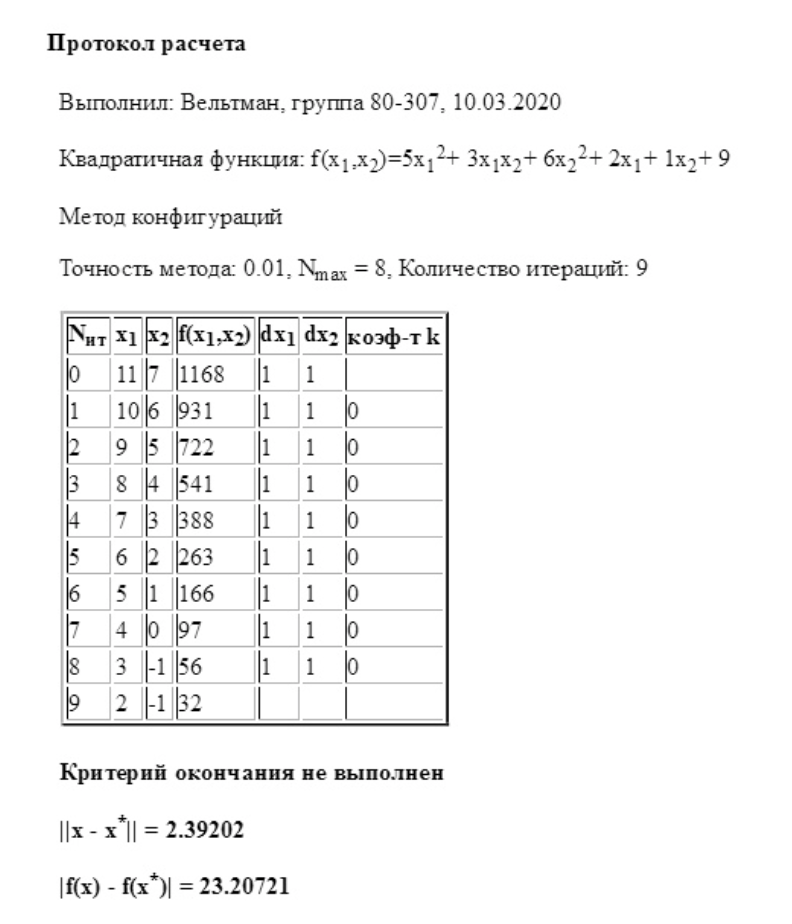
\includegraphics[scale = 0.6]{img/1.PNG}
    
\end{itemize}


\pagebreak

\section{Метод Марквардта}

\begin{itemize}
    \item {\bfseries Класс задач:} безусловная оптимизация
    
    
    \item {\bfseries Формулировка задачи:} Найти минимум функции 2-ух переменных $f(x_1, x_2)$ методом Марквардта.
    
    
    \item {\bfseries Что вычисляется в процессе решения:}
    В процессе иттерации для поиска точки $x^{k+1}$ с меньшим значением функции $f(x)$ вычислятся шаг-приращение $dx^k$ для точки $x^k$ при помощи градиента и матрицы Гёссе в этой точке.
    
    
    \item {\bfseries Алгоритм:}
    Перед началом описания алгоритма следует ввести следующие обозначения: \\
    Матрица Гёссе:
    \begin{equation*}
    H_{f}(x) = \left(
    \begin{array}{cccc}
        \frac{\partial^2 f(x)}{\partial x^{2}_{1}} & \frac{\partial^2 f(x)}{\partial x_1 \partial x_2} & \ldots & \frac{\partial^2 f(x)}{\partial x_1 \partial x_n}\\
        \frac{\partial^2 f(x)}{\partial x_{2} \partial x_1} & \frac{\partial^2 f(x)}{\partial x^{2}_{2}} & \ldots & \frac{\partial^2 f(x)}{\partial x_2 \partial x_n}\\
        \vdots & \vdots & \ddots & \vdots\\
        \frac{\partial^2 f(x)}{\partial x_n \partial x_1} & \frac{\partial^2 f(x)}{\partial x_n \partial x_2} & \ldots & \frac{\partial^2 f(x)}{\partial x^{2}_{n}}
    \end{array}
    \right)
    \end{equation*}
    
    Градиент:
    \begin{equation*}
    \nabla f(x) = \left(
    \begin{array}{cccc}
        \frac{\partial f(x)}{\partial x_1}\\
        \frac{\partial f(x)}{\partial x_2}\\
        \vdots\\
        \frac{\partial f(x)}{\partial x_n}
    \end{array}
    \right)
    \end{equation*}
    Функции $f(x)$, где $x = (x_1, x_2, ..., x_n)$. \\
    
    {\it Описание алгоритма:}
    \begin{enumerate}
        \item {\it Начальная инициализация:} Задать точку для начала движения $x^0 = (x^{0}_1, x^{0}_2, ..., x^{0}_n)$, точность приближения $\xi$, необязательный парамметр - максимальное количество иттераций $N_{max}$, а также выбрать значение параметра $\lambda_0$, которое, впрочем, можно задать как $\lambda_0 = 50 \cdot max(h^{0}_{ij})_{0 \leq i,j \leq n}$, где $h^{k}_{ij}$ - элемент матрицы $H_{f}(x^k)$ на $i$-ой строке и $j$-ом столбце. Начиннаем первую иттерацию при $k = 0$.
        
        \item {\it Проверим критерий останова:} Если выполнено основное условие $\|\nabla f(x^k)\| < \xi$ или дополнительное $k = N_{max}$, где $k$ назовем номером иттерации, выходим из алгоритма с результатом $x^k$.
        
        \item {\it Вычисление новой точки:} Вычислим приращение $dx^k = -[H_{f}(x^k) + \lambda_k E]^{-1} \nabla f(x^k)$ и новую точку $x^{k + 1} = x^k + dx^k$. 
        \begin{itemize}
            \item Если $f(x^{k+1}) < f(x^k)$, значит мы успешно нашли новую точку и можем уменьшить значение параметра $\lambda_{k+1}$, например $\lambda_{k+1} = \displaystyle\frac{\lambda_k}{2}$. Положим  $k = k + 1$ и перейдем к шагу $(2)$.
            \item  Если $f(x^{k+1}) \geqslant f(x^k)$, значит поиск неудачен и следует увеличить значение параметра $\lambda_{k}$, например $\lambda_{k} = \lambda_k \cdot 2$. Параметр  $k$ не меняется и повторим шаг $(3)$ для поиска $x^{k+1}$ с новым параметром $\lambda_k$.
        \end{itemize}
    \end{enumerate} 
    
    
    \item {\bfseries 1-ая итерация:} \\
    $f(x_1, x_2) = 5x^{2}_{1} + 3x_{1}x_{2} + 6x^{2}_{2} + 2x_1 + x_2 + 9$ \\ 
    $\xi = 0.01$\\
    $N_{max} = 5$
    $k = 0$ \\
    $x^{0}_1 = 11$, $x^{0}_2 = 7$
    
    \begin{equation*}
    \nabla f(x) = \left(
    \begin{array}{cccc}
        10x_1 + 3x_2 + 2\\
        12x_2 + 3x_1 + 1
    \end{array}
    \right) 
    \end{equation*}
    
    \begin{equation*}
    H_{f}(x) = \left(
    \begin{array}{cccc}
        10 & 3 \\
        3 & 12
    \end{array}
    \right)
    \end{equation*}
    Матрица Гёссе положительно определена, поэтому для ускорения сходмости возьмем небольшой параметр $\lambda_0 = 1$, хотя в общем случае рекоменуется брать значение на порядок больше, чем элементы в матрице Гёссе.
    
    
    {\it Проверим критерий останова:}
    \begin{equation*}
    \|\nabla f(x^k)\| = \left\|\left(
    \begin{array}{cccc}
        133\\
        118
    \end{array}
    \right)\right\| = \sqrt{133^2 + 119^2} = 177.8004 > 0.01 = \xi
    \end{equation*}
    $k = 0 < 5 = N_{max}$, значит критерий останова не выполнен.
    
    {\it Вычислим следующую точку:}
    \begin{equation*}
    dx^k = -[H_{f}(x^k) + \lambda_k E]^{-1} \nabla f(x^k) = \left[
    \left(
    \begin{array}{cccc}
        10 & 3 \\
        3 & 12
    \end{array}
    \right) 
    + 
    \left(
    \begin{array}{cccc}
        \lambda_k & 0 \\
        0 & \lambda_k
    \end{array}
    \right)
    \right]^{-1} 
    \left(
    \begin{array}{cccc}
        133 \\
        118
    \end{array}
    \right) 
    = 
    \left(
        -10.261, -6.709
    \right)
    \end{equation*}
    
    $x^{k+1} = x^k + dx^k = (11, 7) + (-10.261, -6.709) = (0.739, 0.291)$\\
    $f(x^{k+1}) = 12.2598 < 1168 = f(x^k)$ , значит новая точка найдена успешно. \\
    $\lambda_{k+1} = \displaystyle\frac{\lambda_k}{2} = 0.5$ \\
    $k = k + 1$ \\
    {\it Конец первой итерации.}
    
    \item {\bfseries Результат компьютерных вычислений:} \\
    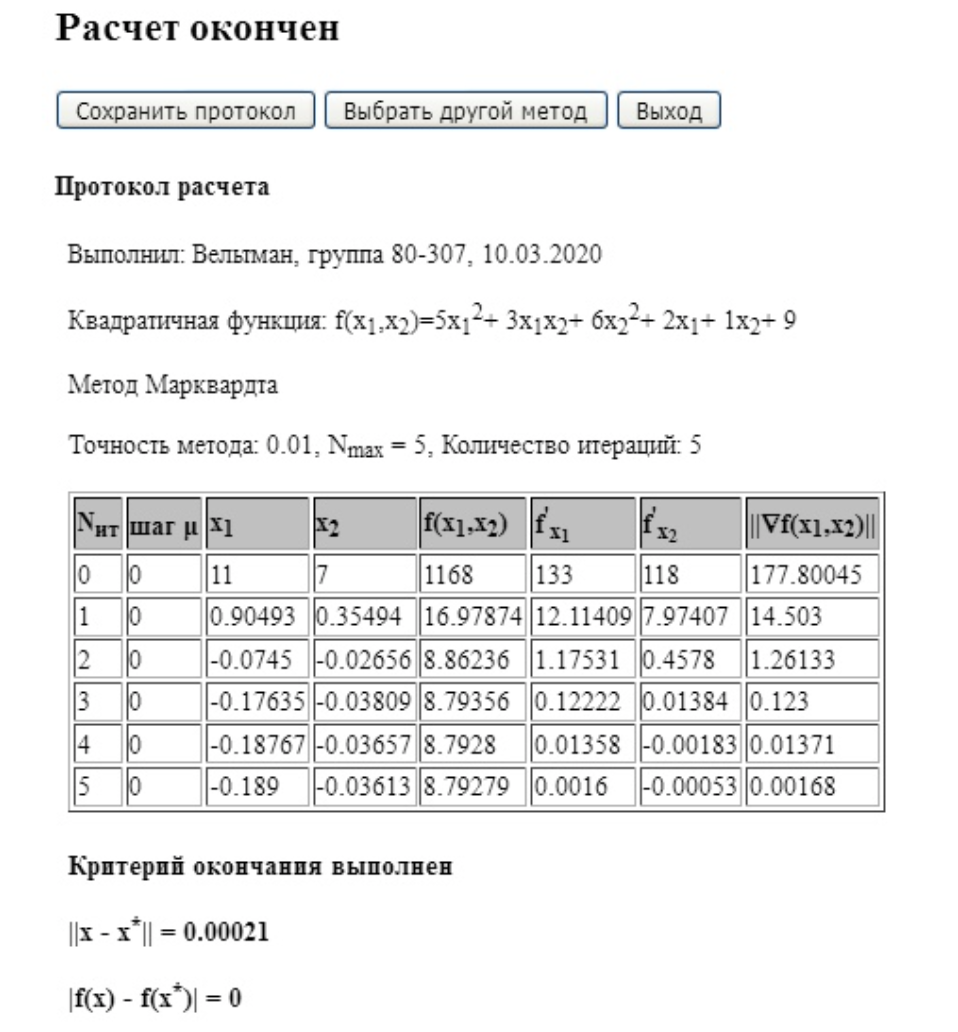
\includegraphics[scale = 0.6]{img/2.PNG}
    
\end{itemize}

\pagebreak

\section{Метод Нелдера-Мида}

\begin{itemize}
    \item {\bfseries Класс задач:} безусловная оптимизация
    
    
    \item {\bfseries Формулировка задачи:} Найти минимум функции 2-ух переменных $f(x_1, x_2)$ методом Нелдера-Мида.
    
    
    \item {\bfseries Что вычисляется в процессе решения:}
    В процессе итераций вычисляется центр тяжести набора точек, с целью заменить \enquote{худшую} точку из набора на более близкую к минимуму функции.
    
    \item {\bfseries Алгоритм:}
    Минимизируем функцию $f(x)$, где $x = (x_1, x_2, ..., x_n)$ \\
    {\it Описание алгоритма:}
    \begin{enumerate}
        \item {\it Начальная инициализация:} Задать начальную систему из $n+1$ точек (многогранник): $\{x^{0(1)}, x^{0(2)}, ..., x^{0(n+1)}\}$, точность $\xi$, максимальное количество иттераций $N_{max}$. Начинаем первую итерацию при $k = 0$.
        
        \item Вычисляется значение функции во всех точках многогранника и выбирается:\\
        	лучшая точка $x^{(l)}: f(x^{(l)}) = \underset{i}{\operatorname{min}}[f(x^{k(i)})]$\\
        	худшая точка $x^{(x)}: f(x^{(x)}) = \underset{i}{\operatorname{max}}[f(x^{k(i)})]$\\
        Далее заданная система точек перестраивается, для этого:
         
        \item {\it Найдем центр тяжести:} Найдем центр тяжести $x^{(c)} = \displaystyle\frac{(\sum\limits^{n+1}_{i=1} x^{k(i)} - x^{x})}{n}$\\
        (для функции 2-х переменных точка $x^{(c)}$ - середина отрезка, соединяющего точки за исключением худшей) 
        
        \item {\it Отражение точки:} Получим точку отражения $x^{(otr)} = (1 + \alpha)x^{(c)} - \alpha x^{x}$.\\

        здесь $ \alpha > 0$ - параметр отражения (рекомендуемое значение $\alpha = 1$)

        \item Формируется новая система точек (многогранник). Для этого в точке $x^{(otr)}$ вычисляется значение функции, полученное значение сравнивается с $f(x^{(l)})$:
        \begin{itemize}
            \item Если $f(x^{(otr)}) < f(x^{(l)})$, значит выполняется операция \underline{растяжение}:\\

            $x^{(rst)} = x^{(c)} + \gamma(x^{(otr)} - x^{(c)})$\\

            здесь $\gamma > 0$ $(\gamma \neq 0)$ - параметр растяжения (рекомендованное значение $\gamma \in [2, 3])$
            При этом, если $f(x^{(rst)}) < f(x^{(otr)})$, то в новой системе точек точка $x^{(x)}$ будет заменена на $x^{(rst)}$, если же $f(x^{(rst)}) \geqslant f(x^{(otr)})$, то в новой системе точек точка $x^{(x)}$ будет заменена на $x^{(otr)}$.

            \item Если $f(x^{(l)}) \leqslant f(x^{(otr)}) < f(x^{(x)})$ выполняется операция \underline{сжатие}:\\

            $x^{(szh)} = x^{(c)} + \beta(x^{(x)} - x^{(c)})$\\

            здесь $\beta > 0$  $(\beta \neq 0)$ - параметр сжатия (рекомендованное значение $\beta \in [0.4, 0.6]$).\\

            При этом, если $f(x^{(szh)}) < f(x^{(otr)})$, то в новой системе точек точка $x^{(x)}$ будет заменена на $x^{(szh)}$, если $f(x^{(szh)}) \geqslant f(x^{(otr)})$, то в новой системе точек точка $x^{(x)}$ будет заменена на $x^{(otr)}$.

            \item Если $f(x^{(otr)}) \geqslant f(x^{(x)})$ выполняется операция \underline{редукции}:\\

            	при этом формируется новый многогранник, содержащий точку $x^{(l)}$ с уменьшенными вдвое сторонами: \\

            		$x^{k + 1(i)} = x^{(l)} + 0.5(x^{k(i)} - x^{(l)}), i = 1, ... , n + 1$\\

            Таким образом, в результате выполнения этого пункта алгоритма формируется новая система точек(многогранник), причем в случае возникновения операций растяжения и сжатия перестраивается только одна точка - $x^{(x)}$, в случае возникновения операции редукции - все точки, за исключением $x^{(l)}$.

        \end{itemize}

        \item Процедура 2) - 5) повторяется до выполнения критерия окончания счета
        
    \end{enumerate} 

    \item \underline{Критерий останова:} Обозначим $\overline{f} = \displaystyle\frac{\displaystyle\sum\limits^{n+1}_{j=1} f(x^{k(j)})}{n + 1}$. \\ 
        Если $\sqrt{\displaystyle\frac{\displaystyle\sum\limits^{n+1}_{i=1} \left|f(x^{k(i)}) - \overline{f}\right|^2}{n + 1}} < \xi$ или $k = N_{max}$, то выходим из алгоритма с значением $x_l$, иначе $k = k + 1$.
    
    \item {\bfseries 1-ая итерация:} \\
    $f(x_1, x_2) = 5x^{2}_{1} + 3x_{1}x_{2} + 6x^{2}_{2} + 2x_1 + x_2 + 9$ \\ 
    $\xi = 0.01$\\
    $N_{max} = 5$
    $k = 0$ \\
    $x^{0}_1 = 11$, $x^{0}_2 = 7$\\
    $\alpha = 1$, $\gamma = 2.8$, $\beta = 0.5$\\
    $x^{0(1)} = (-3, 3),$ $x^{0(2)} = (-3, -2)$, $x^{0(3)} = (11, 7)$\\
    
    {\it Выберем 3 точки:} \\
    $x_l = (-3, 3)$, $x_h = (11, 7)$, $x_g = (-3, -2)$ \\
    
    {\it Найдем центр тяжести:} \\
    $x_c = \displaystyle\frac{x_l + x_g}{2} = (\displaystyle\frac{-3 - 3}{2}, \displaystyle\frac{3 - 2}{2}) = (-3, 0.5)$\\
    
    {\it Отражение точки:} \\
    $x_r = (1 + \alpha)x_c - \alpha x_h = (-6, 1) - (11, 7) = (-17, -6)$\\
    $f(x_r) = 1936$ \\
    $f(x_r) > 1168 = f(x_h)$ , значит делаем сжатие. \\
    
    {\it Сжатие точки:} \\
    $x_s = \beta x_h + (1 - \beta)x_c = (5.5, 3.5) + (-1.5, 0.25) = (4, 3.75)$\\
    $f(x_s) = 230.125$ \\
    $f(x_s) < 1168 = f(x_h)$, значит заменяем точку $x^{k(3)} = x_h$ в наборе на точку $x_s = (4, 3.75)$. \\
    
    {\it Проверим критерий окончания:}\\
    $f(x^{k(1)}) = 78$, $f(x^{k(2)}) = 88$, $f(x^{k(3)}) = 230.125$ \\
    $\overline{f} = \displaystyle\frac{78 + 88 + 230.125}{3} = 132.041667$\\
    
    $\sqrt{\displaystyle\frac{\displaystyle\sum\limits^{3}_{i=1} \left|f(x^{k(i)}) - \overline{f}\right|^2}{n + 1}} = 69.4754403 > 0.01 = \xi$ \\
    $k = 0 < 5 = N_{max}$ \\
    $k = k + 1$\\
    
    {\it Конец первой итерации.}
    
    \item {\bfseries Результат компьютерных вычислений:} \\
    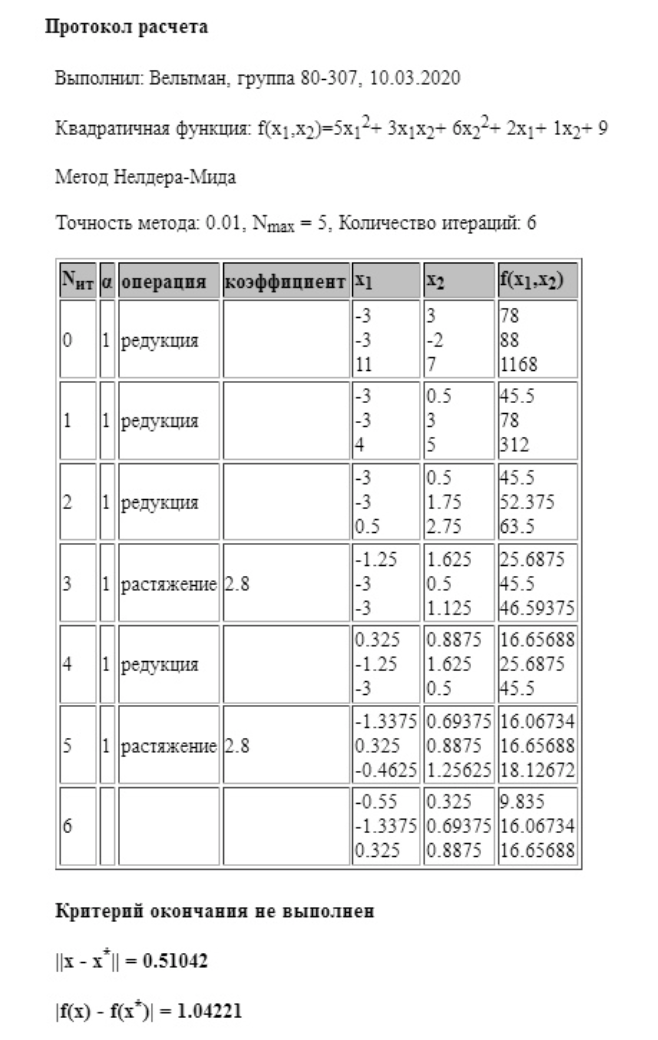
\includegraphics[scale = 0.55]{img/3.PNG}
    
\end{itemize}

\pagebreak


\section{Метод сопряженных градиентов}

(Для квадратичных функций метод сопряженных градиентов называется методом Флетчера-Ривса).

\begin{itemize}
    \item {\bfseries Класс задач:} безусловная оптимизация
    
    
    \item {\bfseries Формулировка задачи:} Найти минимум функции 2-ух переменных $f(x_1, x_2)$ методом сопряженных градиентов.
    
    
    \item {\bfseries Что вычисляется в процессе решения:}
    В процессе иттерации для поиска точки $x^{k+1}$ с меньшим значением функции $f(x)$ вычислятся длина шага $t_k$ и его направление $dx^k$ для точки $x^k$ при помощи градиента, направления $dx^{k-1}$ с предыдущей иттерации и метода дихотомии.
    
    
    \item {\bfseries Алгоритм:}
    Перед началом описания алгоритма следует ввести следующие обозначения: \\
    
    Градиент:
    \begin{equation*}
    \nabla f(x) = \left(
    \begin{array}{cccc}
        \frac{\partial f(x)}{\partial x_1}\\
        \frac{\partial f(x)}{\partial x_2}\\
        \vdots\\
        \frac{\partial f(x)}{\partial x_n}
    \end{array}
    \right)
    \end{equation*}
    Функции $f(x)$, где $x = (x_1, x_2, ..., x_n)$. \\
    
    {\it Описание алгоритма:}
    \begin{enumerate}
    
        \item {\it Начальная инициализация:}\\
        	Задать точку для начала движения $x^0 = (x^{0}_1, x^{0}_2, ..., x^{0}_n)$, точность приближения $\xi$, необязательный парамметр - максимальное количество иттераций $N_{max}$, а также выбрать значение параметра точности поиска $\epsilon$ и отрезка $[a, b]$ для расчета длин шагов. Начинаем первую иттерацию при $k = 0$ и $dx^0 = -\nabla f(x^0)$.
        
        \item {\it Длина шага:}\\
        	Найдем длину шага $t_k = \underset{t \in [a, b]}{\operatorname{argmin}}|f(x^k + t \cdot dx^k)|$, поиск значения которой производится методом дихотомии на заданном отрезке $[a, b]$ с точностью $\epsilon$.
        
        \item {\it Вычисление следующей точки:}\\
        	Найдем новую точку $x^{k + 1} = x^k + t_k \cdot dx^k$ и инкрементируем счетчик $k = k + 1$.
        
        \item {\it Основной критерий окончания метода:}\\
        	Если выполнено основное условие $\|\nabla f(x^k)\| < \xi$ или дополнительное $k = N_{max}$, где $k$ - номер иттерации, выходим из алгоритма с результатом $x^k$.
        
        \item {\it Направление поиска:}\\
        	Найдем новое направление движения \\ $dx^k = -\nabla f(x^k) + \beta_{k-1}dx^{k-1}$, где коеффицент $\beta_{k-1} = \displaystyle\frac{\|\nabla f(x^k)\|^2}{\|\nabla f(x^{k-1})\|^2}$ и перейдем к шагу $(2)$.
        
    \end{enumerate} 
    
    
    \item {\bfseries 1-ая итерация:} \\
    $f(x_1, x_2) = 5x^{2}_{1} + 3x_{1}x_{2} + 6x^{2}_{2} + 2x_1 + x_2 + 9$ \\ 
    $\xi = 0.01$\\
    $\epsilon = 0.001$\\
    $[a, b] = [0.05, 0.5]$\\
    $N_{max} = 5$\\
    $k = 0$ \\
    $x^{0}_1 = 11$, $x^{0}_2 = 7$ \\
    
    Градиент функции расчитывается по формуле:\\
    \begin{equation*}
    \nabla f(x) = \left(
    \begin{array}{cccc}
        10x_1 + 3x_2 + 2\\
        12x_2 + 3x_1 + 1
    \end{array}
    \right) 
    \end{equation*} \\
    
    
    {\it Найдем направление движения:} \\
    Определим начальное направление движения $dx^0 = -\nabla f(x^k) = (-133, -118)$. \\
    
    
    {\it Найдем длину шага:} \\
    Методом дихотомии с точностью $\epsilon$ на отрезке $[a, b]$ определили оптимальное значение как $t_k = t_0 = 0.0722$.\\

    
    {\it Вычислим следующую точку:} \\
    Найдем новое значение точки: \\
    $x^{k+1} = x^k + t_k \cdot dx^k = (11, 7) + 0.0722 \cdot (-133, -118) = (1.4021, -1.5155)$\\
    И увеличим значение $k = k + 1$ \\
    
    {\it Проверим критерий останова:}
    \begin{equation*}
    \|\nabla f(x^k)\| = \left\|\left(
    \begin{array}{cccc}
        11.4743\\
        -12.9793
    \end{array}
    \right)\right\| = \sqrt{(11.4743)^2 + (-12.9793)^2} = 17.3240 > 0.01 = \xi
    \end{equation*}
    $k = 1 < 5 = N_{max}$, значит критерий останова не выполнен.\\
    
    {\it Конец первой итерации.}
    
    \item {\bfseries Результат компьютерных вычислений:} \\
    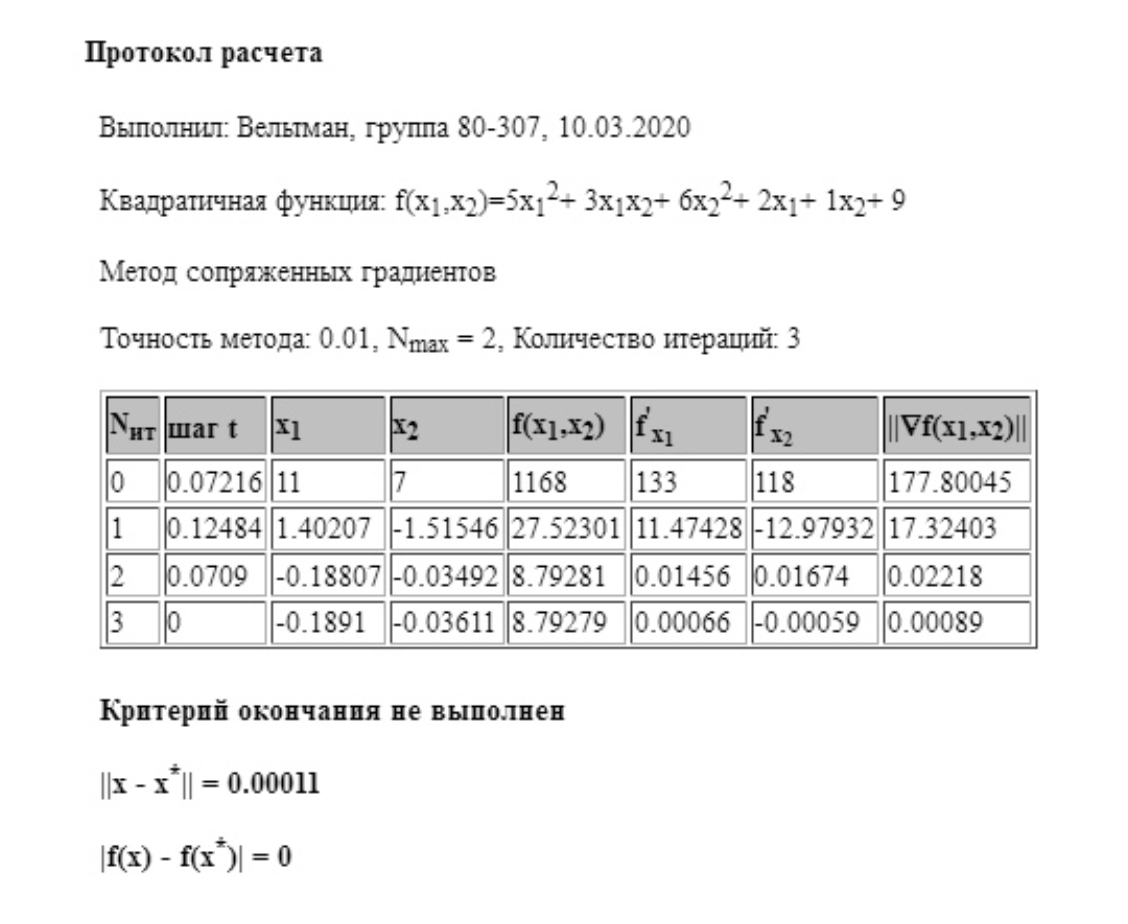
\includegraphics[scale = 0.6]{img/4.PNG}
    
\end{itemize}

\pagebreak


\section{Метод Ньютона-Рафсона}

\begin{itemize}
    \item {\bfseries Класс задач:} безусловная оптимизация
    
    
    \item {\bfseries Формулировка задачи:} Найти минимум функции 2-ух переменных $f(x_1, x_2)$ методом Ньютона-Рафсона.
    
    
    \item {\bfseries Что вычисляется в процессе решения:}
    В процессе иттерации для поиска точки $x^{k+1}$ с меньшим значением функции $f(x)$ вычислятся длина $t_k$ и направление $dx^k$ шага для точки $x^k$ при помощи градиента и матрицы Гёссе в этой точке.
    
    
    \item {\bfseries Алгоритм:}
    Перед началом описания алгоритма следует ввести следующие обозначения: \\
    Матрица Гёссе:
    \begin{equation*}
    H_{f}(x) = \left(
    \begin{array}{cccc}
        \frac{\partial^2 f(x)}{\partial x^{2}_{1}} & \frac{\partial^2 f(x)}{\partial x_1 \partial x_2} & \ldots & \frac{\partial^2 f(x)}{\partial x_1 \partial x_n}\\
        \frac{\partial^2 f(x)}{\partial x_{2} \partial x_1} & \frac{\partial^2 f(x)}{\partial x^{2}_{2}} & \ldots & \frac{\partial^2 f(x)}{\partial x_2 \partial x_n}\\
        \vdots & \vdots & \ddots & \vdots\\
        \frac{\partial^2 f(x)}{\partial x_n \partial x_1} & \frac{\partial^2 f(x)}{\partial x_n \partial x_2} & \ldots & \frac{\partial^2 f(x)}{\partial x^{2}_{n}}
    \end{array}
    \right)
    \end{equation*}
    
    Градиент:
    \begin{equation*}
    \nabla f(x) = \left(
    \begin{array}{cccc}
        \frac{\partial f(x)}{\partial x_1}\\
        \frac{\partial f(x)}{\partial x_2}\\
        \vdots\\
        \frac{\partial f(x)}{\partial x_n}
    \end{array}
    \right)
    \end{equation*}
    Функции $f(x)$, где $x = (x_1, x_2, ..., x_n)$. \\
    
    {\it Описание алгоритма:}
    \begin{enumerate}
        \item {\it Начальная инициализация:}\\
        	Задать точку для начала движения $x^0 = (x^{0}_1, x^{0}_2, ..., x^{0}_n)$, точность приближения $\xi$, необязательный параметр - максимальное количество иттераций $N_{max}$, а также выбрать значение параметра точности поиска $\epsilon$ и отрезка $[a, b]$ для расчета длин шагов. Начинаем первую иттерацию при $k = 0$.
        
        \item {\it Критерий останова:}\\
        	Если выполнено основное условие $\|\nabla f(x^k)\| < \xi$ или дополнительное $k = N_{max}$, где $k$ назовем номером иттерации, выходим из алгоритма с результатом $x^k$.
        
        \item {\it Направление поиска:}\\
        	Найдем новое направление спуска \\ $dx^k = - H^{-1}_{f}(x^k)\nabla f(x^k)$.
        
        \item {\it Длина шага:}\\
        	Найдем длину шага $t_k = \underset{t \in [a, b]}{\operatorname{argmin}}|f(x^k + t \cdot dx^k)|$, поиск значения которой производится методом дихотомии на заданном отрезке $[a, b]$ с точностью $\epsilon$.
        
        \item {\it Вычисление следующей точки:}\\
        	Найдем новую точку $x^{k + 1} = x^k + t_k \cdot dx^k$, инкрементируем счетчик $k = k + 1$ и перейдем к шагу $(2)$.
        
    \end{enumerate} 
    
    
    \item {\bfseries 1-ая итерация:} \\
    $f(x_1, x_2) = 5x^{2}_{1} + 3x_{1}x_{2} + 6x^{2}_{2} + 2x_1 + x_2 + 9$ \\ 
    $\xi = 0.01$\\
    $\epsilon = 0.001$\\
    $[a, b] = [0.05, 0.5]$\\
    $N_{max} = 5$\\
    $k = 0$ \\
    $x^{0}_1 = 11$, $x^{0}_2 = 7$ \\
    
    Градиент:
    \begin{equation*}
    \nabla f(x) = \left(
    \begin{array}{cccc}
        10x_1 + 3x_2 + 2\\
        12x_2 + 3x_1 + 1
    \end{array}
    \right) 
    \end{equation*}
    Матрица Гёссе:
    \begin{equation*}
    H_{f}(x) = \left(
    \begin{array}{cccc}
        10 & 3 \\
        3 & 12
    \end{array}
    \right)
    \end{equation*}\\
    
    
    {\it Проверим критерий останова:}
    \begin{equation*}
    \|\nabla f(x^k)\| = \left\|\left(
    \begin{array}{cccc}
        133\\
        118
    \end{array}
    \right)\right\| = \sqrt{133^2 + 119^2} = 177.8004 > 0.01 = \xi
    \end{equation*}
    $k = 0 < 5 = N_{max}$, значит критерий останова не выполнен. \\
    
    {\it Найдем направление движения:}\\
    \begin{equation*}
    dx^k = -H^{-1}_{f}(x^k)\nabla f(x^k) =
    \left(
    \begin{array}{cccc}
        10 & 3 \\
        3 & 12
    \end{array}
    \right)^{-1} 
    \left(
    \begin{array}{cccc}
        133 \\
        118
    \end{array}
    \right) 
    = 
    \left(
        -11.1913, -7.0408
    \right)
    \end{equation*}
    
    {\it Найдем длину шага:} \\
    Методом дихотомии определили оптимальное значение как $t_k = t_0 = 0.5$.\\
    
    {\it Вычислим следующую точку:}\\
    $x^{k+1} = x^k + t_k \cdot dx^k = (11, 7) + 0.5 \cdot (-11.1913, -7.0408) = (5.4054, 3.4820)$\\
    $f(x^{k+1}) = 298.5946 < 1168 = f(x^k)$, значит новая точка найдена успешно. \\
    $k = k + 1$ \\
    
    {\it Конец первой итерации.}
    
    \item {\bfseries Результат компьютерных вычислений:} \\
    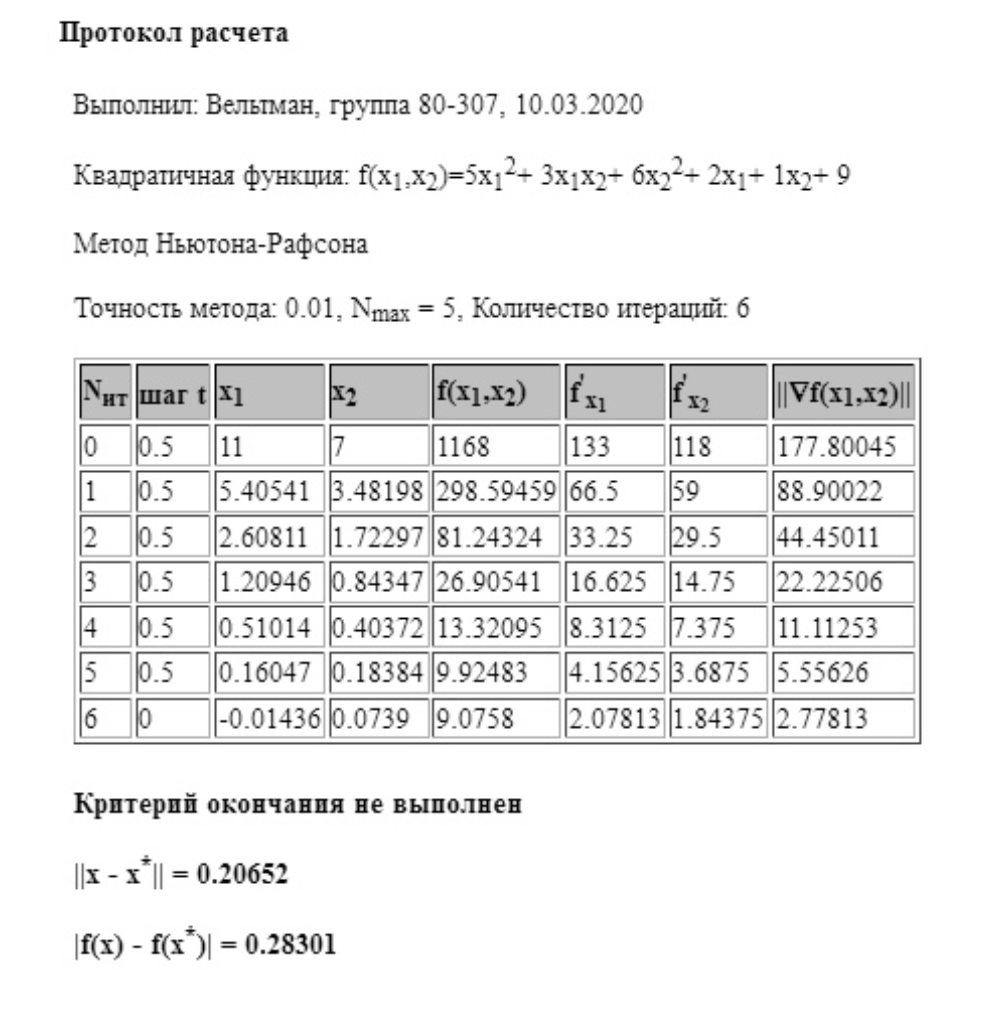
\includegraphics[scale = 0.55]{img/5.PNG}
    
\end{itemize}

\pagebreak